\chapter{RESULTADOS PRELIMINARES}

Este capítulo presenta resultados preliminares de dos componentes de DARL. En
primer lugar, se reporta la tabla de decisión empírica construida con XGBoost
sobre PhysioNet, usada como baseline para comparar estrategias de actualización
selectiva. En segundo lugar, se documenta una demostración práctica del agente
PPO implementada con la librería Stable-Baselines3, cuyo objetivo es validar el ciclo de
decisión POMDP descrito en el Capítulo III, mediante una validación inicial de consistencia
metodológica.

% ------------------------------------------------------------
\section{Baseline empírico de actualización selectiva}
% ------------------------------------------------------------

En el primer experimento se entrena un
\textit{pipeline} de dos etapas con XGBoost como modelo predictivo y se evalúan
cinco estrategias ante drift sintético de distinta naturaleza y severidad. El
AUC del modelo base antes de aplicar las perturbaciones fue $0.7836$; por
ello, la recuperación se reporta como porcentaje relativo respecto a dicho
baseline.

La Tabla~\ref{tab:resultados_baseline_xgboost} resume los resultados principales
de recuperación de AUC. Las acciones A1--A4 corresponden a las estrategias
del espacio de decisión de DARL: diferir, actualizar \textit{features},
actualizar modelo y reentrenar todo. La acción A2c se incluye como estrategia
auxiliar correctiva como alternativa para el feature update. Lo que hace es crear
un \textit{quantile map} que referencia los datos con drift con los originales
para intentar corregir el drift. No forma parte del espacio de
acciones del agente PPO.

\begin{table}[H]
    \centering
    \caption{Baseline empírico XGBoost para actualización selectiva en PhysioNet}
    \label{tab:resultados_baseline_xgboost}
    \scriptsize
    \resizebox{\textwidth}{!}{%
        \begin{tabular}{llrrrrrr}
            \toprule
            \raisebox{-0.7\normalbaselineskip}{\textbf{Condición}} &
            \raisebox{-0.7\normalbaselineskip}{\textbf{Severidad}} &
            \multicolumn{5}{c}{\textbf{\% Recuperación}} &
            \raisebox{-0.7\normalbaselineskip}{\textbf{Acción óptima}} \\
            \cmidrule(lr){3-7}
                                &                    &
            \textbf{A1}         & \textbf{A2}        & \textbf{A2c}          &
            \textbf{A3}         & \textbf{A4}        &                         \\
            \midrule
            Covariate shift     & Leve               & 96.6                   & 95.4  & 95.5  & 98.0  & 98.1  & A1 \\
            Covariate shift     & Moderada           & 90.6                   & 91.8  & 91.8  & 96.6  & 96.7  & A3 \\
            Covariate shift     & Severa             & 84.9                   & 89.7  & 89.8  & 96.1  & 95.7  & A3 \\
            Concept drift       & Leve               & 98.1                   & 100.0 & 100.0 & 99.9  & 100.0 & A2 \\
            Concept drift       & Moderada           & 92.7                   & 82.8  & 92.7  & 96.6  & 96.6  & A1 \\
            Concept drift       & Severa             & 86.3                   & 82.6  & 82.6  & 100.0 & 99.7  & A3 \\
            Covariate + Concept & Moderada           & 87.6                   & 83.1  & 86.4  & 96.6  & 92.9  & A3 \\
            Covariate + Concept & Severa             & 80.8                   & 88.4  & 88.5  & 95.7  & 96.2  & A3 \\
            \bottomrule
        \end{tabular}%
    }
    \vspace{1mm}
    \begin{minipage}{0.96\textwidth}
        \footnotesize
        \textit{Nota.} Rec. indica AUC-ROC de la estrategia dividido entre el
        AUC-ROC baseline ($0.7836$), multiplicado por 100. Los costos relativos
        usados para seleccionar la acción óptima fueron: A1=$0.00x$,
        A2=$0.12x$, A2c=$0.16x$, A3=$0.45x$ y A4=$1.00x$, todos normalizados
        respecto al reentrenamiento completo.
    \end{minipage}
\end{table}


Los resultados muestran que el reentrenamiento completo (A4) no domina
necesariamente la decisión. En drift leve, A1 puede ser óptima porque evita
costo computacional y conserva una recuperación alta. En escenarios moderados o
severos, A3 aparece con frecuencia como mejor compromiso entre recuperación de
AUC y costo relativo: recupera gran parte del desempeño sin pagar el costo total
de A4.

También se observa que la estrategia A2 no siempre mejora el desempeño, aun
cuando el drift contiene componentes covariados. Esto ocurre porque reajustar el
preprocesamiento puede cambiar la representación de entrada sin corregir la
relación aprendida por el modelo. En contraste, A3 es más robusta en los casos
de drift severo o combinado, donde actualizar el modelo predictivo permite
recuperar mejor la relación efectiva entre variables y etiqueta.
Esto ocurre porque el modelo XGBoost realiza una normalización interna
de los datos con drift, mejorando la inferencia del modelo a pesar de la falta
de actualización de los features en A2. Por ello, actualizar el modelo (A3)
tiende a superar a actualizar los features (A2) en casos de Covariate shift.

Esta evidencia preliminar respalda la motivación central de DARL: la
acción de mantenimiento debe elegirse por balance costo-beneficio y no solo por
maximización del rendimiento absoluto. Es decir, la decisión no debe reducirse
a ordenar las acciones por el mayor AUC
recuperado. Si ese fuera el único criterio, el reentrenamiento completo (A4)
tendería a imponerse por ser la acción más exhaustiva; sin embargo, los tiempos
de ejecución normalizados muestran que esta mejora marginal puede no compensar
su costo. En XGBoost, A3 alcanza una recuperación de $96.6\%$ frente a
$96.7\%$ de A4 en \textit{covariate shift} moderado, pero con un costo relativo
de $0.45x$ frente a $1.00x$. Por ello, el criterio relevante para DARL no es escoger la
acción con máximo rendimiento aislado, sino aquella que entrega suficiente
recuperación por unidad de costo computacional.

% ------------------------------------------------------------
\section{Demostración PPO para la aproximación POMDP}
% ------------------------------------------------------------

El segundo resultado corresponde a la demostración de PPO para DARL. Esta
demostración implementa una versión
práctica y liviana del POMDP de DARL usando Stable-Baselines3. El agente no
observa directamente el estado real de las distribuciones, sino un vector
$o_t$ con señales resumidas de severidad, drift, degradación de AUC/F1 y costos
históricos. A partir de esa observación, PPO selecciona una de cuatro acciones:
\textit{Defer}, \textit{Update features}, \textit{Update model} o
\textit{Retrain all}.

\begin{table}[H]
    \centering
    \caption{Hiperparámetros usados en la demo PPO de DARL}
    \label{tab:hiperparametros_ppo_demo}
    \begin{tabular}{ll}
        \toprule
        \textbf{Elemento}                & \textbf{Valor usado}                 \\
        \midrule
        Política                         & \texttt{MlpPolicy}                   \\
        Semilla                          & 42                                   \\
        Longitud de episodio             & 100 pasos                            \\
        Episodios de evaluación final    & 50                                   \\
        Checkpoints de entrenamiento     & 0, 500, 1000, 1500, 2000, 2500, 3000 \\
        Factor de descuento $\gamma$     & 0.95                                 \\
        Peso de recuperación $\lambda_A$ & 1.00                                 \\
        Peso de costo $\lambda_C$        & 0.25                                 \\
        \bottomrule
    \end{tabular}
\end{table}


La evaluación determinística final se realizó sobre 50 episodios de 100 pasos
cada uno, para un total de 5000 decisiones. El reward medio por paso fue
$0.0334$ y el reward acumulado medio por episodio fue $3.3390$ con desviación
estándar $0.4155$. La política final seleccionó principalmente
\textit{Update features} en el $59.86\%$ de los pasos y \textit{Update model} en
el $40.14\%$ restante; no seleccionó \textit{Defer} ni \textit{Retrain all} en
esta evaluación final. Esto indica que, bajo la función de recompensa definida
en la Ecuación~\ref{eq:darl_reward}, los extremos del espacio de acciones
resultan menos atractivos que las actualizaciones selectivas. A1
(\textit{Defer}) tiene costo computacional nulo, pero cuando el drift produce
degradación de AUC no recupera desempeño y por tanto recibe poca recompensa. En
el otro extremo, A4 (\textit{Retrain all}) puede recuperar rendimiento, pero
también concentra el mayor costo de tiempo y memoria; si su ganancia adicional
frente a A2 o A3 es marginal, la penalización de costo reduce su reward neto.
El trade-off aprendido por PPO favorece entonces acciones parciales que
recuperan suficiente desempeño sin pagar el costo completo del reentrenamiento.

\begin{figure}[H]
    \centering
    \subfigure[]{
        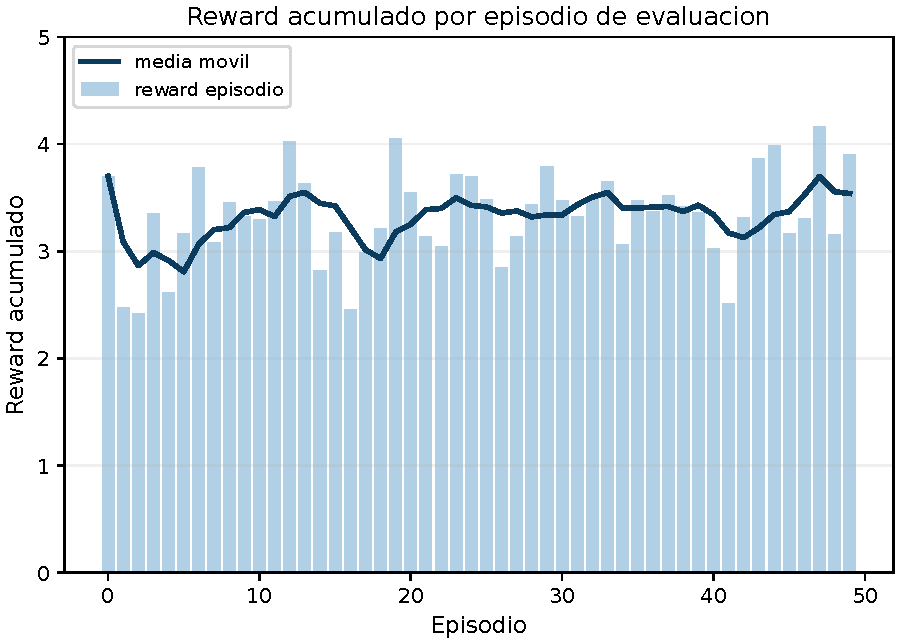
\includegraphics[width=0.47\textwidth]{figures/generated/ppo_reward_episodio.pdf}
    }
    \hfill
    \subfigure[]{
        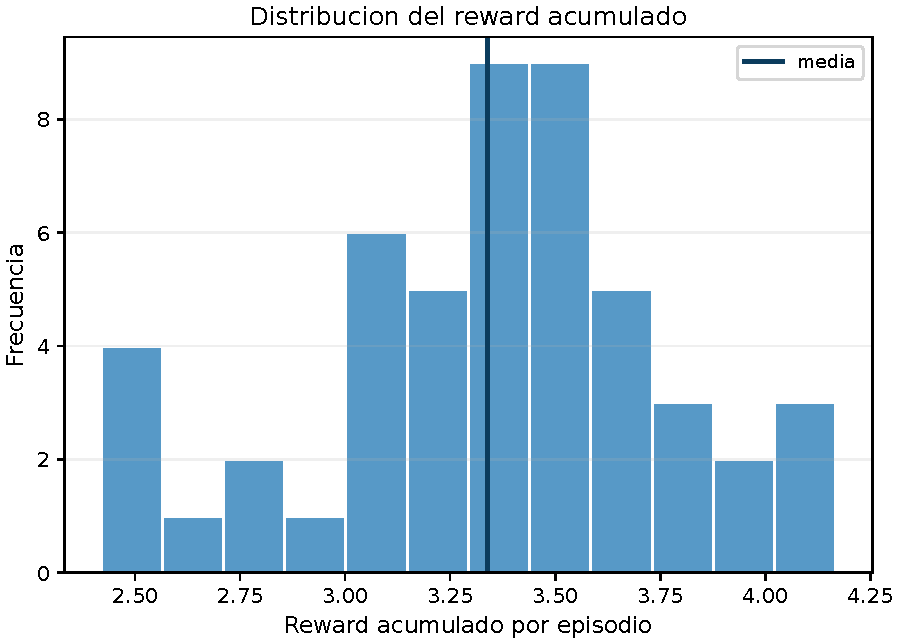
\includegraphics[width=0.47\textwidth]{figures/generated/ppo_reward_distribucion.pdf}
    }
    \caption{Resultados de reward acumulado en la evaluación PPO. La subfigura
        (a) muestra el reward total obtenido en cada episodio junto con una
        media móvil, mientras que la subfigura (b) resume la distribución del
        reward acumulado entre episodios.}
    \label{fig:ppo_reward_episodio_distribucion}
\end{figure}

La Figura~\ref{fig:ppo_reward_episodio_distribucion} resume la variabilidad del
reward acumulado durante la evaluación final. La subfigura (a) muestra el
reward total obtenido en cada episodio y una media móvil que permite observar la
tendencia sin asumir monotonía. La curva se mantiene en valores positivos,
aunque con fluctuaciones, lo cual es esperable porque cada episodio recorre una
secuencia distinta de escenarios sintéticos de drift. En particular, la demo
combina tres condiciones: \textit{covariate shift}, \textit{concept drift} y
drift combinado; cada una aparece con severidad baja, media y alta, codificada
como $0.25$, $0.60$ y $0.90$, respectivamente. Estos escenarios no representan
un único experimento fijo, sino una mezcla controlada de estados donde cambian
las señales de PSI/KS/C2ST, la caída de AUC/F1 y el costo esperado de cada
acción. Por ello, la variación entre episodios refleja que PPO enfrenta
secuencias distintas de tipo y severidad de drift, no ruido de una sola curva de
aprendizaje. La subfigura (b) muestra la distribución del reward acumulado; la
concentración alrededor de valores positivos indica que la política aprendida
tiende a obtener beneficio neto bajo la función de recompensa definida, pero
todavía conserva dispersión entre episodios.

\begin{figure}[H]
    \centering
    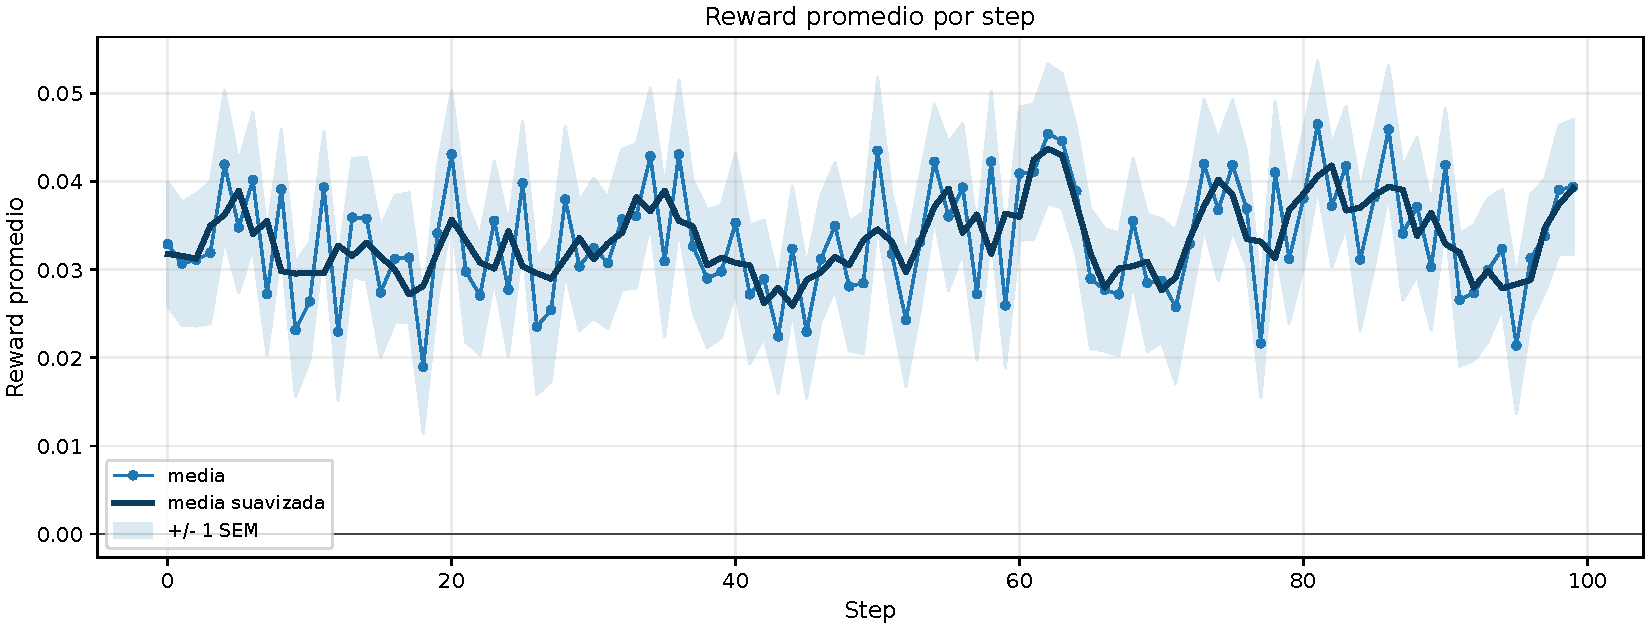
\includegraphics[width=0.98\textwidth]{figures/generated/step_reward_summary.pdf}
    \caption{Reward promedio por paso durante la evaluación PPO}
    \label{fig:ppo_reward_promedio_step}
\end{figure}

La Figura~\ref{fig:ppo_reward_promedio_step} presenta el reward promedio por
paso agregado sobre los 50 episodios. Esta gráfica representa la fase de
inferencia o evaluación determinística de una política PPO ya entrenada, no el
periodo de aprendizaje del agente. Por tanto, no debe interpretarse como una
curva de entrenamiento donde el reward necesariamente aumenta con el tiempo. En
esta demo, cada paso corresponde a un escenario de drift sintético distinto, no
a una dinámica física donde el estado deba mejorar de forma progresiva. Por
ello, las oscilaciones reflejan variabilidad entre escenarios y severidades, así
como la respuesta de la política aprendida ante cada observación. La media
suavizada y la banda de error estándar ayudan a distinguir la señal promedio del
ruido de evaluación.

\begin{figure}[H]
    \centering
    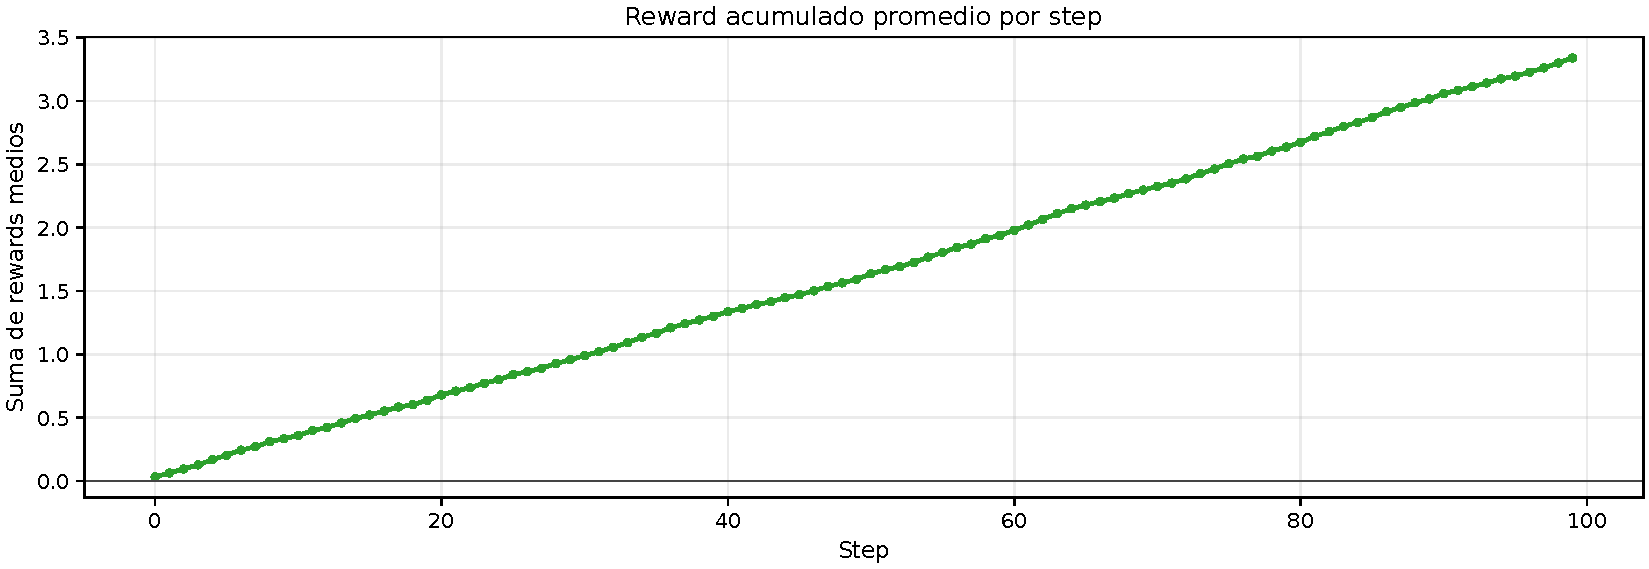
\includegraphics[width=0.98\textwidth]{figures/generated/cumulative_step_reward_summary.pdf}
    \caption{Reward acumulado promedio por paso durante la evaluación PPO}
    \label{fig:ppo_reward_acumulado_step}
\end{figure}

La Figura~\ref{fig:ppo_reward_acumulado_step} muestra la suma acumulada de los
rewards medios por paso. A diferencia del reward puntual, esta visualización
permite observar si la política conserva un beneficio agregado positivo a lo
largo del episodio. La trayectoria creciente indica que, en promedio, las
acciones seleccionadas generan más recuperación ponderada por costo que pérdida
neta. Esta evidencia es coherente con el objetivo práctico de la demo: verificar
que PPO aprende una política útil bajo observaciones parciales, sin forzar una
mejora monotónica del reward en cada paso individual.

% ------------------------------------------------------------
\section{Lectura preliminar}
% ------------------------------------------------------------

En conjunto, los resultados preliminares sugieren que la actualización selectiva
es metodológicamente plausible para DARL. La tabla empírica muestra que la
acción óptima cambia según tipo y severidad de drift, y que el costo computacional
puede cambiar la decisión incluso cuando una estrategia obtiene mayor AUC
absoluto. La demo PPO, por su parte, verifica que un agente puede aprender una
política sobre señales resumidas y seleccionar acciones parciales con reward
positivo promedio. Estos resultados no prueban todavía superioridad frente a
otros métodos, pero sí delimitan la hipótesis que debe validarse: la decisión de
mantenimiento debe depender simultáneamente del tipo de drift, la degradación de
desempeño y el costo relativo de intervenir cada etapa.

Esta lectura también justifica por qué DARL modela el \textit{pipeline} de dos
etapas como una decisión conjunta y no como dos decisiones independientes. La
etapa de preprocesamiento no produce un efecto aislado: al actualizar
\textit{features}, cambia la representación que recibe el modelo predictivo. Por
ello, una corrección de Stage 1 puede reducir señales de \textit{covariate shift},
pero también desalinear al modelo si la relación aprendida entre
variables y etiqueta no se actualiza. De forma análoga, actualizar solo Stage 2
puede ser suficiente ante señales conceptuales, pero no necesariamente corrige
una representación de entrada degradada. El contexto conjunto beneficia la
decisión porque permite evaluar cada acción por su efecto final sobre el
\textit{pipeline} completo: recuperación de AUC/F1, costo de tiempo y memoria, y
compatibilidad entre la representación producida por Stage 1 y la función
predictiva aprendida por Stage 2.

La principal limitación es que la demo PPO usa escenarios sintéticos
deterministas y livianos, diseñados para validar el flujo POMDP y no para
demostrar convergencia definitiva ni superioridad empírica. Como se desprende de
la brecha identificada en el Capítulo I, la validación completa deberá comparar
DARL contra estrategias externas y \textit{baselines} más simples: reentrenar
todo siempre, diferir siempre o aplicar umbrales simples de no acción, actualizar
solo \textit{features} con una regla fija, actualizar solo el modelo con una
regla fija, usar políticas basadas en umbrales de drift/AUC y entrenar un
clasificador supervisado que prediga una de las cuatro acciones a partir de
señales de drift, AUC/F1 y costos. Esa comparación deberá mantener la misma
definición de recuperación de AUC y costo relativo para separar qué parte del
beneficio proviene del contexto de dos etapas y qué parte proviene únicamente de
la regla de decisión usada.
